\documentclass{article}

% if you need to pass options to natbib, use, e.g.:
%     \PassOptionsToPackage{numbers, compress}{natbib}
% before loading neurips_2019

% ready for submission
% \usepackage{neurips_2019}

% to compile a preprint version, e.g., for submission to arXiv, add add the
% [preprint] option:
%     \usepackage[preprint]{neurips_2019}

% to compile a camera-ready version, add the [final] option, e.g.:
     \usepackage[final]{JiyuanLu_Proposal}

% to avoid loading the natbib package, add option nonatbib:
%     \usepackage[nonatbib]{neurips_2019}

\usepackage[utf8]{inputenc} % allow utf-8 input
\usepackage[T1]{fontenc}    % use 8-bit T1 fonts
\usepackage{hyperref}       % hyperlinks
\usepackage{url}            % simple URL typesetting
\usepackage{booktabs}       % professional-quality tables
\usepackage{amsfonts}       % blackboard math symbols
\usepackage{nicefrac}       % compact symbols for 1/2, etc.
\usepackage{microtype}      % microtypography
\usepackage{graphicx}
\usepackage{pdfpages}

\title{Compare N-gram Language Models and Neural Language Models}

% The \author macro works with any number of authors. There are two commands
% used to separate the names and addresses of multiple authors: \And and \AND.
%
% Using \And between authors leaves it to LaTeX to determine where to break the
% lines. Using \AND forces a line break at that point. So, if LaTeX puts 3 of 4
% authors names on the first line, and the last on the second line, try using
% \AND instead of \And before the third author name.

\author{%
  Jiyuan~Lu\\
  Courant Institute of Mathematical Sciences\\
  New York University\\
  New York, NY 10025 \\
  \texttt{jl11046@nyu.edu} \\
  % examples of more authors
  % \And
  % Coauthor \\
  % Affiliation \\
  % Address \\
  % \texttt{email} \\
  % \AND
  % Coauthor \\
  % Affiliation \\
  % Address \\
  % \texttt{email} \\
  % \And
  % Coauthor \\
  % Affiliation \\
  % Address \\
  % \texttt{email} \\
  % \And
  % Coauthor \\
  % Affiliation \\
  % Address \\
  % \texttt{email} \\
}

\begin{document}

\maketitle

\section{Abstract}
Natural Language Generation (NLG), also referred to as text generation, is a subfield of natrual language processing, which leverages knowledge in computational linguistics and artificial intelligence to automatically generate natural language texts. Text categorization, also referred to as text classification, is the task of assigning predefined tags or categories to text according to its content. Under this problem setting, I experimented with two different text generation models and two different text classification models and compared their performance.

\section{Introduction}
As a paricular application of NLG, automatically generating text that mimic what a real person says is an interesting yet challenging problem. Thanks to various modeling techniques scientists have developed during the recent years as well as abundant data available on the Internet, letting computers generate almost-real sentences that can easily fool people is no longer a wild dream.

President Donald Trump frequently uses social media, especially Twitter. From his offcial declaration of candidacy in June 2015 through the first two-and-a-half years of his presidency, he tweeted over 17000 times. By this time, the end of 2019, he should have posted many more tweets. Apart from the large quantity of his tweets, Trump's tweets has a very unique writing style. For example, he used an increasingly disengaged style over the course of the campaign - essentially presenting his opinion as facts and ignoring alternative viewpoints. These factors make Trump's tweets an ideal data source for training a text generator.

In this project, I implemented a style-mimicking text generator called Trump-Robot, which automatically generates tweets in the style of President Donald Trump. In the mean time, I will separately train a text classfier that properly distinguishes Trump's tweets and other people's tweets. Then I will use the text classifier to evaluate the performance of the text generator by seeing how the classifier can distinguish text made up by the text generator from real text. Furthermore, as a potential future work, I might consider using Generative Adversarial Network (GAN) to boost the performance of both the text generator and the text classfier.

\section{Related Work}
There are primarily two types of language models for building text generators. One is statistical language models, which use traditional statistical techniques like N-grams, Hidden Markov Models (HMM) and certain linguistic rules to learn the probability distribution of words. Another is neural language models, which emerged recently and have surpassed the statistical language models in their effectiveness, using different kinds of neural networks to model language, including feedforward neural networks, recurrent neural networks and convolutional neural networks.

The underlying mathematics of the n-gram was first proposed by Markov (1913). Shannon (1948) applied n-grams to compute approximations to English word sequences. Based on Shannon's work, Markov models were commonly used in engineering, linguistic, and psychological work on modeling word sequences by the 1950s. Later, Jelinek (1976) at the IBM and Baker (1975) at CMU independently used n-grams in their speech recognition systems with some success. The highest accuracy language models by now are neural network language models, including feedforward language models (Bengio et al. 2006, Schewenk 2007), recurrent language models (Mikolov 2012), and gated convolutional networks language model (Dauphin 2016). They solve a major problem with n-gram language models: the number of parameters increase exponentially as the n-gram order increases, and n-grams have no way to generalize from training to test set. Neural language models instead project words into a continuous space in which words with similar contexts have similar representations.

There are also two primary approaches for building text classifiers. One is rule-based systems, which classify text into organized groups by using a set of handcrafted linguistic rules. These rules instruct the system to use semantically relevant elements of a text to identify relevant categories based on its content. Each rule consists of an antecedent or pattern and a predicted category. Rule-based systems are human comprehensible and can be improved over time, but these systems require deep knowledge of the domain. Also, generating rules for a complex system can be very time-consuming and these systems don't scale well given that adding new rules can affect the results of pre-exisiting rules. Another is machine learning based systems, which learns to make classifications based on past observations instead of relying on manually crafted rules. They are usually much more accurate than human-crafted rule systems, especially on complex classification tasks, and are also easier to maintain and scale by only feeding new tagged training examples to the model to learn new tasks. Some of the most popular machine learning algorithm for creating text classification models include traditional statistical methods like naive bayes (Wang \& Manning 2012), support vector machine (Silva et al., 2011), modified logistic regression (Le \& Mikolov, 2014), and neural network methods, including recursive neural networks (Wermter 2000) and convolutional neural networks (Kalchbrenner et al., 2014, Santos \& Gatti, 2014, Shen et al., 2014).

\section{Dataset}
The first dataset is Trump's tweets, which is easily accessible thanks to various websites maintaining Trump's historic tweets. In particular, I used the dataset from a website called "Trump Twitter Archive". This dataset contains 36307 tweets of Trump from 5/4/2009 to 12/10/2019, among which many are retweets that are actually written by other people. After cleaning, I preserved only 24595 tweets that are written by Trump.  And this dataset is used for training both the text generator and the text classfier.

The second dataset is tweets selected from three politicians and celebrities: Barack Obama, Hillary Clinton, and Kim Kardashian. This dataset is a subset of the "Raw Twitter Tmelines w/ No Retweets" dataset on Kaggle. I will collect the roughly the same amount of tweets as in the Trump tweets dataset, for a number of 24196 tweets, and it is used to train the text classifier only. 

\section{Data Preprocessing}
Two levels of data preprocessing is applied to both datasets. The input to the classifier goes through two processing steps, but the input to the generator goes through only the first processing step. The reason why it is done in two steps is that I would like the classifier to learn slightly different things from the generator. After all, the goal of the classfier is to correctly categorize an input sentence, while the goal of the generator is to generate tweets that look as similar to Trump's as possible.

\subsection{Preprocessing Step 1}
First, as mentioned, all retweets are removed because they are from other people and cannot represent the style of Trump.

Next, quotations, URLs, line feeds, extra whitespaces, and picture links are removed. 

Then, appearances of "\&amp" are replaced with "and".

\subsection{Preprocessing Step 2}
In addition, for training classfiers:

First, characters such as "@" (mention somebody) and "\#" (tag something) are removed, along with other special characters.

Next, "'ll" is replaced by " will", "won't" is replaced by "will not", "n't" is replaced by " not".

Finally, common stop words in English are also removed, except for "no", "not" and "never". Common tweet symbols such as "rt" (meaning retweet) and "cc" (meaning "carbon copy") are also added to the stop word list for removal.

\section{Problem Formulation}
There are two models to design in this project: a text generator for generating made-up tweets in the style of Trump, and a text classifier for distinguishing Trump's tweets from other people's tweets.

For the text generator, two different models are used and compared. First, a traditional word n-gram model is used, including bigram and trigram models. Second, a neural language model is used, i.e., a word-level and long short-term memory (LSTM).

For the text classifier, two models are used and compared. One is Multinomial Naive Bayes and the other is LSTM. The classifier with the highest prediction accuracy on the test set is considered the best classifier and is in turn used to distinguish made-up tweets generated by the text generator from real Trump's tweets.

\section{Evaluation Metric}
There are two models to evaluate in this project: a text generator for generating made-up tweets in the style of Trump, and a text classifier for distinguishing Trump's tweets from other people's tweets.

The text generator is essentially a language model. The best way to evaluate the performance of a language model is to embed it in an application and measure how much the application improves. Such end-to-end evaluation is called extrinsic evaluation. Extrinsic evaluation is the only way to know if a particular improvement in a component is really going to help the task at hand. Thus, for text generation, we can compare the performance of two generators by running a separately trained text classfier to distinguish made-up tweets from real Trump's tweets. The one which better fools the text classifier, i.e., whose made-up tweets yielding lower accuracy on the text classfier is considered a better text generator.

Sometimes running NLP systems end-to-end is very expensive, so another evaluation method, called intrinsic evaluation, can be used to quickly evaluate potential improvements of the model before using a more expensive extrinsic evaluation method. An intrinsic evaluation metric is one that measures the quality of a model independent of any application. For an instrinsic evaluation of the text generator we need a test set, sometimes called held out corpora that are not in our training sets. Therefore, to compare the performance of two text generators, we divide the data into training and test sets, train the parameters of both generators on the training set and then compare how well the two trained models fit the test set. By "fit the test set", we mean the probability that a language model (i.e., text generator) assigns to the test sentence. Whichever model assigns a higher probability to the test set - meaning it more accurately predicts the test set - is a better model. 

However, in practice, perplexity is often used as the metric for evaluating language models instead of raw probability. The perplexity of a language model on a test set is the inverse probability of the test set, normalized by the number of words. It is related inversely to the likelihood of the test sequence according to the language model and can also be thought of as the weighted average branching factor of a language. Therefore, in comparing two text generators, whichever model achieves a lower preplexity on the test set - meaning it gives us more information about the word sequence - is a better model.

The performance of the text classifier is evaluated similarly to the intrinsic evalution of a language model. To compare the performance of two text classifiers, we also divide the data into training and test sets, train the parameters of both classifiers on the training set and then compare how well the two trained models fit the test set. By "fit the test set", we mean the ability to correctly classify the test sentence into its correct category (Trump or Not-Trump). Whichever model achieves a higher prediction accuracy on the test set - meaning it more accurately predicts the category of the test sentence - is a better model.

\section{Model}
\subsection{Text Classifier}
Two different text classifier models are experimented and compared: One is a Multinomial Naive Bayes text classifier, a traditional statistical approach. The other is an LSTM text classifier, a modern neural network approach.
\subsubsection{Multinomial Naive Bayes Text Classifier}
Multinomial Naive Bayes implements the naive Bayes algorithm for multinomially distributed data, and is one of the two classic naive Bayes variants used in text classification (the other is Bernoulli Naive Bayes model, which also assumes multiple features but each feature is binary-valued). The features are usually word vector counts, but tf-idf vectors are also known to work well in practice.

For each class y, the distribution is parameterized by vectors $\theta_y = (\theta_{y1}, ..., \theta_{yn})$, where n is the numer of features (words in the vocabulary). $\theta_{yi}$ is the probability $P(x_i | y)$ of feature i appearing in a sample beloning to class y.

The parameters $\theta_y$ is estimated by a smoothed version of maximum likelihood, i.e., relative frequency counting:  

$\hat{\theta_{yi}} = \frac{N_{yi} + \alpha}{N_y + \alpha n}$  

Here $N_{yi}$ is the number of times feature i appears in a sample of class y in the training set T, and $N_y$ is the total count of all features for class y. $\alpha$ is used as the smoothing priors. By default, $\alpha$ = 1 is used and this is called Laplace smoothing.

The multinomial Naive Bayes classifier is suitable for classification with discrete features and word counts is such an example.

\subsubsection{LSTM Text Classifier}
Long Short Term Memory (LSTM) is an recurrent neural netowork (RNN) architecture that has feedback networks. It was develped to deal with the exploding and vanishing gredient problems that can be encountered when training traditional RNNs. As a variation of RNN, LSTM is well-suited to classifying, processing, and making predictions on serial data.


First, the input tweets (sentences) are tokenized. There are serveral parameters to set for the tokenizer:

1. num words: the maximum number of words to keep, based on word frequency. Only the most common (num words - 1) words will be kept. Default is None, meaning all words will be kept.

2. Filters: a string where each element is a character that will be filtered from the texts. The default is all punctuation, plus tabs and line breaks, minus the ' character.

3. lower: Boolean indicating whether to convert the texts to lowercase. Default is True.

4. split: String indicating the separator for word splitting. The default is ' ' (space).

5. char level: Boolean indicating if every characeter will be treated as a token. Default is False.

6. oov token: String. If given, it will replace out-of-vocabulary words.

I basically followed the default setting except setting the num words field to 50000 to keep the top 49999 words in the vocabulary. I also provided a string "<OOV>" to represent all out of vocabulary words.

Then, each sentence is "standardized" and each word is trasformed into an index in the truncated vocabulary. Any tweet that is longer than 40 words is truncated at the tail, and any tweet that is shorter than 40 words is padded at the tail with value 0.

Finally, we are ready to define our LSTM architecture.  

First, the tokenized sentences are feed into an embedding layer. Weights from GloVe embeddings pretrained on Twitter are used, with an embedding dimension of 200. Every word in a sentence are transformed from an index in the vocabulary to a dense vector of fixed dimension 200. A dropout layer is attached with a dropout probability of 0.4.

Second, two bidirectional LSTM layers with hidden dimension 128 are chained together. A dropout layer is attached to the last LSTM with a dropout probability of 0.2.

Third, a dense layer with hidden dimension 128 using ReLU activation function is applied. A dropout layer is attached with a dropout probability of 0.4.

Fourth, a dense layer with hidden dimension 64 using ReLU activation function is applied. A dropout layer is attached with a dropout probability of 0.5.

Finally, a sigmoid activation function is applied to generate a number between 0 and 1 representing the output probability of label 1.

\subsection{Generator}
Two different text generator models are experimented and compared: One is a Markov chain (n-gram) text generator, a traditional statistical approach. The other is an LSTM text generator, a modern neural network approach.
\subsubsection{Markov Generator}
Two different Markov generator are experimented and compared: One is a bigram language model, the other is a trigram language model.
\subsubsubsection{Bigram Text Generator}
A bigram is a sequence of two adjacent elements from a string of tokens. It helps provide the conditional probability of a token given the preceding token, when the relation of conditional probability is applied:

$P(W_n | W_{n-1}) = \frac{P(W_{n-1}, W_n)}{P(W_{n-1})}$

That is, the probability P of a token $W_n$ given the preceding token $W_{n-1}$ is equal to the probability of their bigram, or the co-occurrence of the two tokens $P(W_{n-1}, W_n)$, divided by the probability of the preceding token.

\subsubsubsection{Trigram Text Generator}
A trigram is a sequence of three adjacent elements from a string of tokens. It helps provide the conditional probability of a token given the two preceding tokens, when the relation of conditional probability is applied:

$P(W_n | W_{n-1}, W{n-2}) = \frac{P(W_{n-2}, W_{n-1}, W_n)}{P(W_{n-2}, W_{n-1})}$

That is, the probability of a token $W_n$ given the preceding tokens $W_{n-1}$ and $W_{n-2}$ is equal to the probability of their trigram, or the co-occurrence of the three tokens,  $P(W_{n-2}, W_{n-1}, W_n)$, divided by the probability of the co-occurrence of the preceding two tokens,  $P(W_{n-2}, W_{n-1})$.

\subsubsection{LSTM Generator}
Three bidirectional LSTMs with hidden size set to 256 are stacked together. Up to 8 previous words are considered before generating the next word. A maximum of 10000 words are modeled, the rest with lower frequencies are ignored. And no dropout is applied.
\section{Experiments}
\subsection{Text Classifier}
Data is shuffled and split into 80\% test set 10\% validation set and 10\% test set.

Naive Bayes classifier is chosen as the final text classifier to descriminate the fake sentences generated by text generators since it has a higher test accuracy.
\subsubsection{Multinomial Naive Bayes Text Classifier}
10-fold cross validation is used to tune the hyperparameters of the text classifier. For a Multinomial Naive Bayes text classification model, the hyperparameters are:  

1. N-gram range: (1, 1), (1, 2), (1, 3), (2, 2), (2, 3), (3, 3). They correspond to using only (word) unigram; using unigram and bigram; using unigram, bigram, and trigram; using only bigram; using bigram and trigram; using only trigram, respectively.  

2. Using tf-idf: True or False. True means we are using tf-idf vectors as features, while False means we are using smoothed word counts as features.

3. Tf-idf norm: L1 or L2. L1 norm means each output row (for an input instance) will have sum of squares of vector elements of 1, while L2 norm means sum of absolute values of vector elements is 1.  

4. Alpha: 1, 0.1, 0.01. Alpha represents the additive smoothing coefficient.

Precision is used as the metric for evaluating and thus choosing the model in cross validation. Precision is chosen instead of accuracy because I want a classifier that is strict when labeling an input instance as Trump. In this way, it won't be easily fooled by the fake Trump sentences generated by the text generator.

After cross validation, the best hyperparameters of the model are: Using unigram, bigram and trigram, using raw counts instead of tf-idf, and using a smoothing coefficient of 0.1.

Here is an image showing the performance of the Naive Bayes classifier model: The non-Trump tweets are labeled 0 and the Trump tweets are labeled 1. For non-Trump tweets, the precision is 0.9325, the recall is 0.9376, and the F1-score is 0.9350. For Trump tweets, the precision is 0.9368, the recall is 0.9316, and the F1-score is 0.9342. The model performs almost equally well on the two class labels, with precision of the Trump tweet category a bit higher than the non-Trump tweet, but at the expense of recall, and therefore the F1-score.

\begin{figure}
\centering
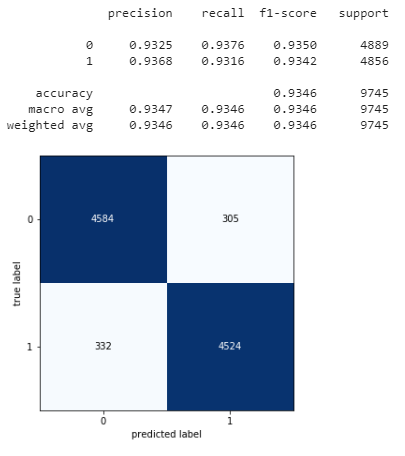
\includegraphics{img/CLF_NB.PNG}
\end{figure}

\subsubsection{LSTM Text Classifier}
Quite suprisingly, compared to the simple Naive Bayes model, the LSTM model performs a bit worse.

Here is an image showing the performance of the LSTM classifier model: The non-Trump tweets are labeled 0 and the Trump tweets are labeled 1. For non-Trump tweets, the precision is 0.8977, the recall is 0.9172, and the F1-score is 0.9074. For Trump tweets, the precision is 0.9185, the recall is 0.8992, and the F1-score is 0.9087. The model performs almost equally well on the two class labels, with precision of the Trump tweet category a bit higher than the non-Trump tweet, but at the expense of recall.

\begin{figure}
\centering
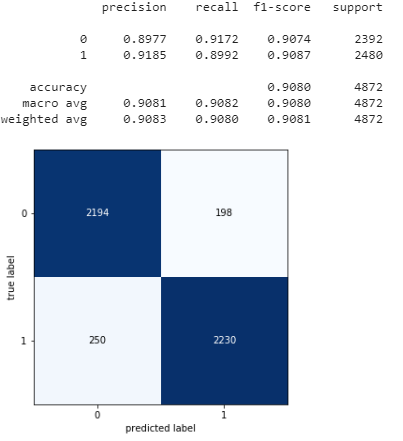
\includegraphics{img/CLF_LSTM.PNG}
\end{figure}

\subsection{Generator}
\subsubsection{Markov Generator}
\subsubsubsection{Bigram Text Generator}
Intrinsic evaluation: 

The best tweet, i.e., the tweet generated by the bigram text generator having the highest probability under the Trump language model, has a probability of 1.0000. And the sentence is: 

\textit{From a large shipment of military weapons and supplies to my GREAT members at Trump International Golf Links in Scotland!}.

The 75\% percentile tweet has a probability of 0.9849 and is written:

\textit{Watch it, should be ashamed for using the celebrity’s name followed by new champion Chris Weidman!}

The median percentile tweet has a probability of 0.9406 and is written:

\textit{\#Debates .USA has the guts to even greater unemployment.}

Extrinsic evaluation: Provide the Naive Bayes text classifier with 1000 fake Trump tweets generated by the bigram text generator, 93\% of them successfully fooled the classifier, meaning that they are falsely recognized by the classifier as real Trump tweets.

\subsubsubsection{Trigram Text Generator}
The best tweet, i.e., the tweet generated by the bigram text generator having the highest probability under the Trump language model, has a probability of 1.0000. And the sentence is: 

\textit{The Rigged Witch Hunt headed by 13 Angry Democrats and others who are totally corrupt and/or conflicted.}

The 75\% percentile tweet has a probability of 0.9876 and is written:

\textit{Thank you, a very wise move that Ted Cruz FORGOT to file.}

The median percentile tweet has a probability of 0.9555 and is written:

\textit{In the meantime they continue to be drawn to it.}

Extrinsic evaluation: Provide the Naive Bayes text classifier with 1000 fake Trump tweets generated by the bigram text generator, 94.7\% of them successfully fooled the classifier, meaning that they are falsely recognized by the classifier as real Trump tweets.

\subsubsection{LSTM Generator}
The best tweet, i.e., the tweet generated by the bigram text generator having the highest probability under the Trump language model, has a probability of 1.0000. And the sentence is: 

\textit{fundraisers have zero credibility on china , its economy and would have been 3 \% since the witch hunt is totally rigged and corrupt . where the fake news media is going crazy !}

The 75\% percentile tweet has a probability of 0.9956 and is written:

\textit{words and has a after the two - fake news ! cnn just doesn ’ t work much harder than it is and to win . all of our " i never said " " clinton " " was}

The median percentile tweet has a probability of 0.9846 and is written:

\textit{weakness while she was secretary of state , has terrorists all over the world . . cont : " once again @ barackobama is self - play the veterans day . big speech in florida and florida}

Notice that the sentences are truncated if they are too long.

Extrinsic evaluation: Provide the Naive Bayes text classifier with 1000 fake Trump tweets generated by the bigram text generator, 99.5\% of them successfully fooled the classifier, meaning that they are falsely recognized by the classifier as real Trump tweets.

\section{Conclusion}
1. A simple traditional Naive Bayes model outperforms an expensive LSTM model on the text classfication task for distinguishing Trump's tweet's from other people's tweets. 

2. The n-gram langauge models generate more "reasonable" (by human) fake Trump tweets than the LSTM does, in which a trigram model has better performance both intrinsically and extrinsically than a bigram model. However, the LSTM generator can fool the classifier better.

3. Both n-gram generators and LSTM generators can fool the classifier well, making it almost unable to distinguish the fake Trump tweets from the real Trump tweets.

\section*{References}
\small

[1] Jurafsky, D., and Martin, J.H. (2019).  N-gram Language Models. Speech and Language Processing (third edition draft). 

[2] Shannon, C. E. (1948). A mathematical theory of communication. Bell System Technical Journal, 27(3), 379–423.

[3] Jelinek, F. (1976). Continuous speech recognition by statistical methods. Proceedings of the IEEE, 64(4), 532–557.

[4] Baker, J. K. (1975). The DRAGON system – An overview. IEEE Transactions on Acoustics, Speech, and Signal Processing, ASSP-23(1), 24–29.

[5] Bengio, Y., Schwenk, H., Senecal, J.-S., Morin, F., and Gauvain, J.-L. (2006). Neural probabilistic language models. In Innovations in Machine Learning, 137–186. Springer.

[6] Schwenk, H. (2007). Continuous space language models. Computer Speech \& Language, 21(3), 492–518.

[7] Mikolov, T. (2012). Statistical language models based on neural networks. Ph.D. thesis, Ph. D. thesis, Brno University of Technology.

[8] Dauphin, Y.N., Fan, A., Auli, M., and Grangier D. (2016). Language Modeling with Gated Convolutional Networks. Computation and Language. arXiv:1612.08083.

[9] Jeffreys, H. (1948). Theory of Probability (2nd Ed.). Clarendon Press. Section 3.23.

[10] Johnson, W. E. (1932). Probability: deductive and inductive problems (appendix to). Mind, 41(164), 421–423.

[11] Kneser, R. and Ney, H. (1995). Improved backing-off for Mgram language modeling. In ICASSP-95, Vol. 1, 181–184.

[12] Chen, S. F. and Goodman, J. (1998). An empirical study of smoothing techniques for language modeling. Tech. rep. TR-10-98, Computer Science Group, Harvard University.

[13] Wang, S., and Manning, C. D. (2012). Baselines and bigrams: Simple, good sentiment and topic classification. In Proceedings of the 50th Annual Meeting of the Association for Computational Linguistics: Short Papers-Volume 2 (pp. 90-94). Association for Computational Linguistics.

[14] Silva, J., Coheur, L., Mendes, A. C., and Wichert, A. (2011). From symbolic to sub-symbolic information in question classification. Artificial Intelligence Review, 35(2), 137-154.

[15] Le, Q. V., and Mikolov, T. (2014). Distributed representations of sentences and documents. arXiv:1405.4053.

[16] Wermter, S. (2000). Neural network agents for learning semantic text classification. Information Retrieval, 3(2), 87-103.

[17] Kalchbrenner, N., Grefenstette, E., and Blunsom, P. (2014). A Convolutional Neural Network for Modelling Sentences. Acl, 655665.

[18] Santos, C. N. dos, and Gatti, M. (2014). Deep Convolutional Neural Networks for Sentiment Analysis of Short Texts. In COLING-2014 (pp. 6978).

[19] Shen, Y., He, X., Gao, J., Deng, L., and Mesnil, G. (2014). A Latent Semantic Model with Convolutional-Pooling Structure for Information Retrieval. Proceedings of the 23rd ACM International Conference on Conference on Information and Knowledge Management CIKM 14, 101110.

[20] Dickens, M. (2016). “I Have the Best Classifiers”: Identifying Speech Imitating the Style of Donald Trump. CS224d Deep Learning for Natural Language Processing course project reports, Stanford University.



\end{document}